%%%%%%%%%%%%%%%%%%%%%%% file template.tex %%%%%%%%%%%%%%%%%%%%%%%%%
%
% This is a general template file for the LaTeX package SVJour3
% for Springer journals.          Springer Heidelberg 2010/09/16
%
% Copy it to a new file with a new name and use it as the basis
% for your article. Delete % signs as needed.
%
% This template includes a few options for different layouts and
% content for various journals. Please consult a previous issue of
% your journal as needed.
%
%%%%%%%%%%%%%%%%%%%%%%%%%%%%%%%%%%%%%%%%%%%%%%%%%%%%%%%%%%%%%%%%%%%
%
% First comes an example EPS file -- just ignore it and
% proceed on the \documentclass line
% your LaTeX will extract the file if required
\begin{filecontents*}{example.eps}
%!PS-Adobe-3.0 EPSF-3.0
%%BoundingBox: 19 19 221 221
%%CreationDate: Mon Sep 29 1997
%%Creator: programmed by hand (JK)
%%EndComments
gsave
newpath
  20 20 moveto
  20 220 lineto
  220 220 lineto
  220 20 lineto
closepath
2 setlinewidth
gsave
  .4 setgray fill
grestore
stroke
grestore
\end{filecontents*}
%
\RequirePackage{fix-cm}
%
%\documentclass{svjour3}                     % onecolumn (standard format)
%\documentclass[smallcondensed]{svjour3}     % onecolumn (ditto)
\documentclass[smallextended]{svjour3}       % onecolumn (second format)
%\documentclass[twocolumn]{svjour3}          % twocolumn
%
\smartqed  % flush right qed marks, e.g. at end of proof
%
\usepackage{graphicx}

%
% \usepackage{mathptmx}      % use Times fonts if available on your TeX system

% insert here the call for the packages your document requires
%\usepackage{latexsym}
% etc.
%
\usepackage{amsmath}		% AMS Math (http://www.ams.org/tex/amslatex.html)
\usepackage{amssymb}		% AMS Symbols
%\usepackage{amsthm}			% AMS Theorems
\usepackage{tocloft}		% Format the Table of Contents
\usepackage{float}			% More float commands
%\usepackage{sectsty}		% Format section and chapter headings
\usepackage{graphicx}		% Insert images in eps or pdf format
\usepackage{setspace}		% Line-spacing

\usepackage[utf8]{inputenc}
\usepackage{graphicx}
%\usepackage{setspace}
%\doublespacing
\usepackage{algorithm}
\usepackage[noend]{algpseudocode}
\usepackage{color}
\usepackage{tcolorbox}
\usepackage{amsmath}
\usepackage{float}% http://ctan.org/pkg/float
\usepackage{gensymb}
\usepackage{makeidx}  % allows for indexgeneration
\usepackage{amssymb}
\usepackage{graphicx}
\usepackage{mathrsfs}

\usepackage{mathrsfs}
%\usepackage{nd3}
\usepackage{pgf}
\usepackage{multirow,array}
\usepackage{mathpartir}
\usepackage{float}
\usepackage{tikz}
\usetikzlibrary{arrows,automata,positioning,shapes.multipart}
\usepackage{stmaryrd}

%\usepackage{natbib}
\usepackage{fancyvrb}
%\usepackage{microtype}
\usepackage{alltt}
\usepackage{listings}

%\newtheorem{theorem}{Theorem}[section]
%\newtheorem{lemma}[theorem]{Lemma}
%\newtheorem{corollary}{Corollary}[theorem]
%\newtheorem{definition}{Definition}[theorem]
% please place your own definitions here and don't use \def but
% \newcommand{}{}
\newcommand{\Rel}[1]{R_{#1}}
\newcommand{\Act}[1]{[ \mathit{#1} ]}
\newcommand{\ActPos}[1]{\langle \mathit{XSTIT_{#1}} \rangle}
\newcommand{\Know}{\mathbf{K}\,} 
\newcommand{\Kns}[1]{\mathbf{K}_{\mathbf{#1}}\,} 
\newcommand{\Bel}{\mathbf{B}\,} 
\newcommand{\Bels}[1]{\mathbf{B}_{\mathbf{#1}}\,} 
\newcommand{\Pos}  {\langle \mathbf{K} \rangle\,} 
\newcommand{\Poss}[1]  {\langle \mathbf{K}_{#1} \rangle\,}
\newcommand{\BPos} {\langle \mathbf{B} \rangle\,}
\newcommand{\BPoss}[1]{\langle \mathbf{B}_{#1} \rangle\,}
\newcommand{\STIT}[1] {\mathbf{[XSTIT\ {#1}]}}
\newcommand{\Safe} {\mathbf{S}}
\newcommand{\safe} {\mathit{safe}}
\newcommand{\choice}[1]{\mathit{Choice_{#1}}}
\newcommand{\neXt}{\mathit{X}}
\newcommand{\Pal}[1]{\mathbf{[#1]}}
\newcommand{\PalPos}[1]{\mathbf{\langle#1\rangle}}
\newcommand{\SPal}[1]{\mathbf{[#1]^\mathcal{S}}}
%	\stackrel{\mathbf{safe}}{\mathbf{[#1,#2]}}}
\newcommand{\SPalPos}[1]{\mathbf{\langle#1\rangle^\mathcal{S}}}
%
\newcommand{\etal}{\textit{et.~al.}}
\newcommand{\nnot}{\textsf{\ not \ }}
\newcommand{\oor}{\textsf{\  or \ }}
\newcommand{\iiff}{{\  \Leftrightarrow \ }}
\newcommand {\aand}{ \textsf{\ and \ } }
\newcommand {\timplies} { \textsf{\ implies \ }}
\newcommand {\tland}{{\ \wedge \ }}
\newcommand {\tlor}{{\ \vee \ }}
\newcommand {\tlnot}{{\neg}}
\newcommand {\iimplies}{{\ \Rightarrow \ }}

\newenvironment{proofenum}{%                                     
	\begin{enumerate}
		\renewcommand\labelenumi{(\arabic{section}.\arabic{enumi})}}
	{\end{enumerate}}

% Insert the name of "your journal" with
% \journalname{myjournal}
%
\begin{document}

\title{L\"ob-safe Logic for Human-like Agents%\thanks{Grants or other notes
%about the article that should go on the front page should be
%placed here. General acknowledgments should be placed at the end of the article.}
}
%\subtitle{A bi-modal solution}

%\titlerunning{Short form of title}        % if too long for running head

\author{Seth Ahrenbach         \and
        Second Author %etc.
}

%\authorrunning{Short form of author list} % if too long for running head

\institute{F. Author \at
              first address \\
              Tel.: +123-45-678910\\
              Fax: +123-45-678910\\
              \email{fauthor@example.com}           %  \\
%             \emph{Present address:} of F. Author  %  if needed
           \and
           S. Author \at
              second address
}

\date{Received: date / Accepted: date}
% The correct dates will be entered by the editor


\maketitle

\begin{abstract}
L\"ob's Obstacle is a problem facing agents who can reason with certain powers of self-reference. When epistemic logics model the reasoning of human-like agents, they model agents that have such powers. This paper shows L\"ob's Obstacle in various formal systems of epistemic logic, and presents an epistemic logic that avoids it by relaxing assumptions about agents' knowledge and belief. 
\keywords{L\"ob's Theorem \and Epistemic Logic \and Agent Foundations}
% \PACS{PACS code1 \and PACS code2 \and more}
% \subclass{MSC code1 \and MSC code2 \and more}
\end{abstract}

\section{Introduction}
\label{intro}
Epistemic logic emerged from attempts to formalize philosophers' theories of knowledge. It has since found usefulness in areas of computer science ranging from database theory to artificial intelligence and information security. In economics, it serves as a foundation for the ideally rational agents of game theory. These applications tend to treat knowledge as a metaphorical concept relating information to things that can be modeled as agents, even if they are not very complex. While recent advances concerning the combination of dynamic logics with epistemic notions demonstrate the liveliness of the field, the static foundation of these dynamic logics has not advanced beyond the elegant S5 modal operator in quite some time. 

This paper argues that philosophical logicians must return their attention to the static base. Lying at the core of epistemic logic is an obstacle emerging from the depths of mathematical logic that threatens to undermine the enterprise. This obstacle blocks the way forward of any epistemic logic intended to model reasonably sophisticated agents, and certainly those for modeling humans and advanced artificial intelligence. It has many names, but researchers in the field of Agent Foundations call it L\"ob's Obstacle. This paper describes how L\"ob's Obstacle prevents epistemic logics of various sorts from modeling human-like agents, and then describes a logic that is L\"ob Safe which combines weakened knowledge and belief operators into a multi-modal system.

Section \ref{sec:modal_section} reminds readers of the basics of modal logic and its epistemic interpretation. In section \ref{sec:lob_section} we present the modal version of L\"ob's Theorem and describe its importance for mathematical logic. Section \ref{sec:crashing_logics} identifies a number of logics from the epistemic modal family and shows how each one collides with L\"ob's Obstacle, rendering them inapplicable to reasonably complex agents. Section \ref{sec:avoid_lob} presents an epistemic logic that avoids L\"ob's Obstacle by weakening the knowledge and belief operators. We mount a defense of this logic on philosophical grounds while also identifying its flaws. We hope to spark a conversation that will improve the state of epistemic logic's foundation so that it can model cognitive attitudes of humans and advanced machine intelligence. Section \ref{sec:conclusion} concludes with suggested criteria for assessing potential formal epistemic solutions.


\section{Modal Logic}
\label{sec:modal_section}
Modal logic extends propositional logic with simple syntax, but the increase in expressive power is quite dramatic. Initially explored by Aristotle, picked up again by Medieval philosophers, and finally revived in the early 20th century, modal logic's intended inperpretation is as a logic of necessary and possible truths. But this is not the only interpretation of the symbols. By fiddling with the semantics of the modal operators, one can create a modal logic for reasoning in a wide variety of aspects. In the late 1950's and 60's, renewed interest in modal logic for reasoning about temporal modalities led to alternative interpretations, like logic of oblication (deontic logic), logic of knowledge and belief (epistemic and doxastic logics), and provability logic. Each of these logics is a modal logic with different interpretations of the modal operator, and different constraints on the underlying possibility relations.

This paper explores the way modal logics for belief, knowledge, and provability run into a fundamental mathematical obstacle of self-referential reasoning, or even just reasoning with fixed points, which inevitably leads to corrupted inferences. Ironically, the modal formula capturing the obstacle was first identified in deontic logic, illustrating the cross-cutting nature of modal logic.

\section{L\"ob's Theorem}
\label{sec:lob_section}
L\"ob's Obstacle takes its name from Martin Hugo L\"ob, who answered one of L. Henkin's follow up questions to G\"odel's striking incompleteness theorems. The question was, ``what about formulas that assert their own \emph{provability}, as opposed to unprovability?"\footnote{Not a direct quote.} L\"ob's response was as follows. A sufficiently powerful system, \emph{e.g.} Peano arithmetic, can prove that formulas asserting that their own provability implies that they are true only when Peano arithmetic actually proves the formula. It seems a little trivial. For formal systems capturing the reasoning of agents, it can lead to surprising results.

L\"ob's Theorem in provability logic is,
\begin{center}~\label{lob}
	\begin{equation}
		\Box(\Box\varphi \iimplies \varphi)\iimplies \Box\varphi.
	\end{equation}
\end{center}
The $\Box$ is interpreted as ``provability" in some formal system, particularly one at least as powerful as Peano arithmetic. If a modal operator involves the reasoning abilities of a human-like agent, then \emph{a fortiori} it is a formal system at least as powerful as Peano arithmetic. This presents the following problem. If that agent, in its own reasoning system, can deduce the soundness of its own system, then it's reasoning system is unsound. This is because $\varphi$ can be any formula, including $\bot$. The particular modal logic at risk, in our mind, is epistemic logic, or any doxastic logic with accurate reasoners.

%L\"ob identified the following conditions of a formal system that would allow derivation of his theorem (which we present in modal form).
%\begin{enumerate}
%	\item $\Box(\varphi \iimplies \psi) \iimplies (\Box\varphi \iimplies \Box \psi)$\mbox{}\hfill Axiom K
%	\item $\Box\varphi \iimplies \Box\Box\varphi$ \mbox{}\hfill Axiom 4
%	\item From $\vdash \varphi$, infer $\Box\varphi$ \mbox{}\hfill Rule of Necessitation
%\end{enumerate}
%
%Items (1) and (3) are costants for all normal modal logics. There is a suppressed condition that L\"ob did not mention because it was unnecessary for the domain of arithmetic, but we must mention it here. The system must either admit of self-referential sentences or involve modal fixed points. Because systems of human-like reasoning must include self-referential sentences, at least in the form of Peano arithmetic, in order to remain human-like, this condition is satisfied for our concerns. 

Here we give a template derivation of L\"ob's Theorem, which we shall refer to below when describing how L\"ob's Obstacle corrupts various epistemic logics.

\begin{proofenum}
	\item $\Box(\Box\varphi \iimplies \varphi)$\mbox{}\dotfill Assumption
	\item $\Box(\psi \iiff (\Box\psi\iimplies \varphi))$\mbox{}\dotfill L\"ob Sentence\footnote{Sometimes referred as a Curry sentence after Logician Haskell Curry.}
	\item $\Box(\Box\psi \iiff \Box(\Box\psi \iimplies \varphi))$\mbox{}\dotfill Axiom K
	\item $\Box(\Box\psi \iimplies \Box(\Box\psi \iimplies \varphi)))$\mbox{}\dotfill (4.3) Simplification of $\iiff$
	\item $\Box(\Box\psi \iimplies (\Box\Box\psi \iimplies \Box\varphi))$\mbox{}\dotfill (4.4) Axiom K
	\item $\Box(\Box\psi \iimplies \Box\Box\psi)$\mbox{}\dotfill Axiom 4
	\item $\Box(\Box\psi \iimplies \Box\varphi)$\mbox{}\dotfill (4.5), (4.6)
	\item $\Box(\Box\psi \iimplies \varphi)$\mbox{}\dotfill (4.7), (4.1)
	\item $\Box\psi$\mbox{}\dotfill (4.3), (4.8)
	\item $\Box\Box\psi$\mbox{}\dotfill (4.9), Axiom 4
	\item $\Box\Box\psi \iimplies \Box\varphi$\mbox{}\dotfill (4.8), Axiom K
	\item $\Box\varphi$\mbox{}\dotfill (4.10), (4.11)
\end{proofenum}\mbox{}\hfill $\mathcal{QED}$

Mathematical and Provability logicians refer to the key components of this proof as L\"ob Conditions. Identifying them in the proof above helps us identify which epistemic logics collide with L\"ob's Obstacle. Conversely, understanding how the L\"ob Conditions interact helps us construct epistemic logics that avoid the Obstacle.

The Conditions are:
\begin{enumerate}
	\item The L\"ob Sentence. A self-referential sentence, also formalizable as a modal fixed point.
	\item Axiom K. The standard distribution axiom of normal modal logics.
	\item Axiom 4. The axiom corresponding to a transitive frame relation.
	\item The rule of necessitation. Likewise a standard feature of normal modal logics.
\end{enumerate} 

The L\"ob Sentence is sometimes not mentioned as a Condition, because L\"ob's Theorem is typically studied in the context of mathematical logic or provability logic, where such self-referential expressiveness is known to exist. We point out, however, that humans are capable of reasoning about self-referential sentences, as well, and any advanced artificial agent will be able to do so, as well. 

Finally, we note the importance of L\"ob's Theorem's antecedent: $\Box(\Box\varphi \iimplies \varphi)$. Epistemic logics typically include the antecedent as a theorem, in which case L\"ob's Theorem will allow us to derive $\Box\varphi$ for all $\varphi$. This is why consistent mathematical systems at least as expressive as Peano arithmetic cannot prove their own consistency. 

We identify some candidate epistemic logics and, on the assumption that they capture human-like reasoning, show how they crash into L\"ob's Obstacle.

\section{Epistemic Logics that Crash}
\label{sec:crashing_logics}
\subsection{S5 Epistemic Logic}
The most prominent epistemic logic in the literature, by far, is S5 epistemic logic. S5 epistemic logic is routinely presented as the logic of knowledge, and often serves as a static base for dynamic extensions to epistemic logic involving action and communication. Its characteristic axioms are:
\begin{eqnarray}
	\Kns{i}(\varphi \iimplies \psi)\iimplies (\Kns{i}\varphi \iimplies \Kns{i}\psi)\\
	\Kns{i}\varphi \iimplies \varphi\\
	 \tlnot\Kns{i}\varphi \iimplies \Kns{i}\tlnot\Kns{i}\varphi
\end{eqnarray}
Clearly (2) is Axiom K, and (3), troublingly, is the antecedent of L\"ob's Theorem, known as Axiom T. (4) is called the Negative Introspection axiom, or sometimes in philosophy circles, the Wisdom Axiom. Logicians call it Axiom 5. It is read, ``If $i$ does not know that $\varphi$, then she knows that she doesn't know it". Other than being clearly invalid for humans, this axiom and (3) allows us to derive,
\begin{equation*}
	\Kns{i}\varphi \iimplies \Kns{i}\Kns{i}\varphi
\end{equation*}
\begin{proof}
	$\\$
\begin{proofenum}
    \item $\tlnot\Kns{i}\tlnot\Kns{i}\varphi \iimplies \Kns{i}\varphi$\mbox{}\hfill Contrapositive of Axiom 5
    \item $\Kns{i}\tlnot\Kns{i}\tlnot\Kns{i}\varphi \iimplies \Kns{i}\Kns{i}\varphi$\mbox{}\hfill Rule of Necessitation on (5.1), Axiom K
    \item $\varphi \iimplies \tlnot\Kns{i}\tlnot \varphi$\mbox{}\hfill Axiom T, Contrapositive
    \item $\tlnot\Kns{i}\tlnot\varphi \iimplies \Kns{i}\tlnot\Kns{i}\tlnot\varphi$\mbox{}\hfill Axiom 5
    \item $\varphi \iimplies \Kns{i}\tlnot\Kns{i}\tlnot \varphi$\mbox{}\hfill (4.3), (4.4)
    \item $\Kns{i}\varphi \iimplies \Kns{i}\tlnot\Kns{i}\tlnot\Kns{i}\varphi$\mbox{}\hfill $\Kns{i}\varphi$/$\varphi$, (4.5)
    \item $\Kns{i}\varphi\iimplies\Kns{i}\Kns{i}\varphi$\mbox{}\hfill (4.2), (4.6)
	
\end{proofenum}\mbox{}\hfill$\mathcal{QED}$
\end{proof}

Thus, S5 satisfies L\"ob's three conditions, if we assume the presence of self-referential sentences possible, which we should. Therefore, with $\Kns{i}$ instead of $\Box$, the proof of L\"ob's Theorem is possible in this brand of S5. However, to make matters worse, the antecedent of L\"ob's Theorem is itself an axiom of S5. Therefore, $\Kns{i}\varphi$ is a theorem, for all $\varphi$.

We take this as a \emph{reductio ad absurdum} that S5 epistemic logic cannot be a logic for reasoning about the knowledge of agents with expressive power beyond Peano arithmetic. Therefore, it cannot be a logic of knowledge for humans, or human-like agents.

\subsection{Hintikka's S4 Epistemic Logic}
\label{sec:hint_s4}
In Hintikka's 1967 \emph{Knowledge and Belief: A logic of the two notions}, he presented an epistemic logic for determining the validity and consistency of claims people make about knowledge and belief. He rejected out of hand the negative introspection axiom for knowledge, but chose to include positive introspection, which is formalized as $\Kns{i}\varphi\iimplies\Kns{i}\Kns{i}\varphi$. Clearly then, if Hintikka's epistemic system is meant for human-like reasoners who can express sentences like, ``If I know this sentence is true, then 1 + 1 = 2," then it crashes into L\"ob's Obstacle, with the extra bite of having the antecedent of L\"ob's Theorem as a theorem itself, and therefore, $\Kns{i}\varphi$ is also a theorem.

\section{Bi-Modal Synthesis of Knowledge and Belief}
\label{sec:bimodals}

\subsection{Hintikka's Bi-Modal System}
\label{sec:hint_bimodal}

\subsection{Kraus and Lehman System}
\label{sec:kl}

\subsection{Voorbraak's Objective Knowledge and Rational Belief: OKRIB}
\label{sec:okrib}

\section{CRAP}
\label{sec:crap}

\begin{table}[H]
\begin{center}
	\begin{tabular}{| l r |}
		\hline
		$\Kns{i}(\varphi \iimplies \psi) \iimplies (\Kns{i}\varphi \iimplies \Kns{i}\psi)$ & Distribution of $\Kns{i}$ \\
		$\Kns{i}\varphi \iimplies \varphi$ & Truth \\
		$\Bels{i}(\varphi \iimplies \psi) \iimplies (\Bels{i}\varphi \iimplies \Bels{i}\psi)$ & Distribution of $\Bels{i}$\\
		$\Bels{i}\varphi \iimplies \BPoss{i}\varphi$ & Belief Consistency \\
%		$\Bels{i}\varphi \iimplies \Bels{i}\Bels{i}\varphi$ & Positive Belief Introspection \\
%		$\tlnot\Bels{i}\varphi \iimplies \Bels{i}\tlnot\Bels{i}\varphi$ & Negative Belief Introspection\\
		$\Kns{i}\varphi \iimplies \Bels{i}\varphi$ & Knowledge implies Belief \\
		$\Bels{i}\varphi \iimplies \Bels{i}\Kns{i}\varphi$ & Evidential Restraint\\
		%			$\Bels{i}\varphi \iimplies \Kns{i}\Bels{i}\varphi$ & Beliefs are Known\\
		From $\vdash \varphi$ and $\vdash \varphi \iimplies \psi$, infer $\vdash\psi$ & Modus Ponens\\
		From $\vdash \varphi$, infer $\vdash \Kns{i}\varphi$ & Necessitation of $\Kns{i}$\\
		\hline
	\end{tabular}
	\caption{Logic of Grounded-Coherent Epistemic Agents}~\label{GC_agent}
\end{center}
\end{table}

%
%The operators in this logic are reduced in power relative to other logics of knowledge and belief. Here, knowledge is true, belief is consistent, knowledge implies belief, beliefs are subjectively justified, and both operators are normal modal operators. Knowledge lacks both epistemic introspection properties, while belief has positive introspection. As with all normal epistemic operators, these suffer from the problem of logical omniscience, which this paper does not attempt to solve. Rather, we shall show that in the instance of knowledge, the L\"obian Obstacle is avoided. The positive introspection property of belief is a theorem, however, so L\"ob's Theorem will be derivable for the belief operator.
\begin{theorem}[Positive Belief Introspection]~\label{belief_posint}
	$\Bels{i}\varphi \iimplies \Bels{i}\Bels{i}\varphi$
\end{theorem}
\begin{proof}
	$\\$
	\begin{proofenum}
		\item $\Bels{i}\varphi \iimplies \Bels{i}\Kns{i}\varphi$\mbox{}\hfill ER Axiom
		\item $\Bels{i}\Kns{i}\varphi \iimplies \Bels{i}\Bels{i}\varphi$\mbox{}\hfill KiB Axiom + Necessitation of $\Bels{i}$\footnote{This rule can be derived from Necessitation of $\Kns{i}$ and KiB Axiom.}
		\item $\Bels{i}\varphi \iimplies \Bels{i}\Bels{i}\varphi$\mbox{}\hfill (5.1), (5.2)
	\end{proofenum}
\end{proof}\mbox{}\hfill $\mathcal{QED}$

The logic defined by these axiom schemas and inference rules avoids L\"ob's Obstacle for $\Kns{i}$, as it is no longer has the positive introspection property.

\begin{figure}[H]
	\begin{center}
		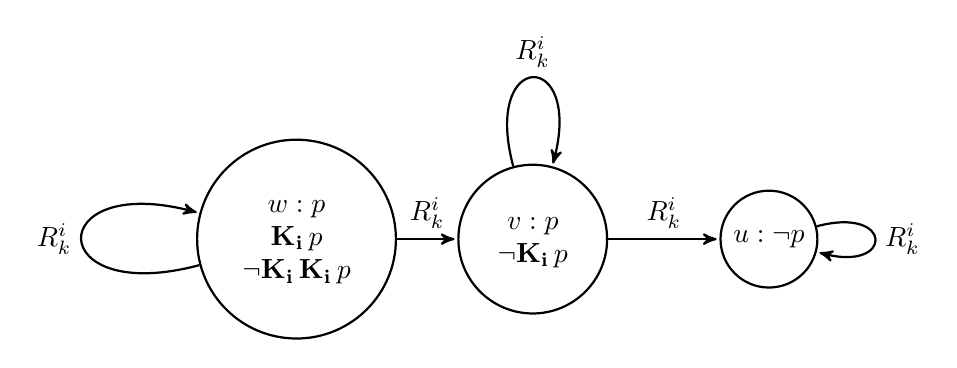
\begin{tikzpicture}[->,>=stealth',shorten >=1pt,auto,node distance=3cm,
		thick,base node/.style={circle,draw,minimum size=35pt}]
		
		\node[base node] (w) {\begin{tabular}{c}
			$w:  p$ \\ $\Kns{i}p$ \\ $\tlnot\Kns{i}\Kns{i}p$
			\end{tabular}};
		\node[base node] (v) [right of=w] {\begin{tabular}{c}
			$v:  p$ \\ $\tlnot\Kns{i}p $
			\end{tabular}};
		\node[base node] (u) [right of=v] {$u: \tlnot p$};
		\path[]
		(w) edge node[above] {$\Rel{k}^i$} (v)
		edge [loop left] node {$\Rel{k}^i$} (w)
		(v) 
%		edge node[below] {} (w)
		%	\draw [->] (v) edge[in=5,out=355,loop] node[right] {$R$} (v)
		edge [<-, loop above] node {$\Rel{k}^i$} (v)
		edge node[above] {$\Rel{k}^i$} (u)
		(u)  edge [<-, loop right] node {$\Rel{k}^i$} (u);
		\end{tikzpicture}
	\end{center}
	\caption{A counterexample to $\Kns{i}\varphi\iimplies\Kns{i}\Kns{i}\varphi$.}
\end{figure}
%
%This logic also avoids the disaster of L\"ob's Theorem for belief, because $\Bels{i}(\Bels{i}\varphi \iimplies \varphi)$ is no longer a theorem.
%
%\begin{figure}[H]
%	\begin{center}
%		\begin{tikzpicture}[->,>=stealth',shorten >=1pt,auto,node distance=3.4cm,
%		thick,base node/.style={circle,draw,minimum size=35pt}]
%		
%		\node[base node] (w) {\begin{tabular}{c}
%			$w:  p$ \\ $\BPoss{i}(\Bels{i}p \tland \tlnot p)$
%			\end{tabular}};
%		\node[base node] (v) [right of=w] {\begin{tabular}{c}
%			$v:  \tlnot p$  \\
%			$\Bels{i}p$
%			\end{tabular}};
%		\node[base node] (u) [right of=v] {$u:  p$};
%		\path[]
%		(w) edge node[above] {$\Rel{k,b}^i$} (v)
%		edge [loop left] node {$\Rel{k}^i$} (w)
%		(v) 
%		%		edge node[below] {} (w)
%		%	\draw [->] (v) edge[in=5,out=355,loop] node[right] {$R$} (v)
%		edge [<-, loop above] node {$\Rel{k}^i$} (v)
%		edge node[above] {$\Rel{k,b}^i$} (u)
%		(u)  edge [<-, loop right] node {$\Rel{k,b}^i$} (u);
%		\end{tikzpicture}
%	\end{center}
%	\caption{A counterexample to $\Bels{i}(\Bels{i}\varphi \iimplies \varphi)$.}~\label{not_conceited}
%\end{figure}
%
%Therefore, L\"ob's Theorem has the same effect for belief as it does for Peano arithmetic: $i$ believes that her belief is accurate only for propositions that she actually believes. Her belief in her own accuracy is not a general claim. In this light, its effect is mitigated, in the same way it is for arithmetic. Because L\"ob's antecedent is not valid for belief, $i$ is not what Smullyan calls a \emph{conceited} reasoner. With L\"ob's Theorem for belief, $i$ constitutes what Smullyan calls a \emph{modest} reasoner.
%
%How shall we interpret the $\BPoss{i}$ operator? Figure \ref{not_conceited} could be read ``it is consistent with what $i$ believes that $i$ falsely believes that $p$". It is somewhat standard to interpret knowledge and belief operators in this way: ``...consistent with what $i$ knows/believes".  We do not endorse this interpretation due to the smell of circularity hanging around it. We prefer the interpretation ``$i$ considers it possible that..." for $\BPoss{i}$ and ``$i$ has evidence that..." for $\Poss{i}$. 
%
%If we consider the contrapositive of L\"ob's Theorem for belief, it states $\tlnot \Bels{i} \varphi \iimplies \tlnot\Bels{i}(\Bels{i} \varphi \iimplies \varphi)$. Indeed, this is G\"odel's Second Incompleteness Theorem applied to belief: ``if $i$ does not believe $\varphi$, then $i$ does not believe that believing $\varphi$ implies its truth." If we substitute in $BPoss{i}$ for $\tlnot\Bels{i}\tlnot$ and push the negation into the implication, the consequent is $\BPoss{i}(\Bels{i}\varphi \tland \tlnot \varphi)$, which is the formula illustrated in Figure \ref{not_conceited}. We read this as ``$i$ considers it possible that she believe $p$ but $p$ be false. This is perhaps a bit strange. However, the interpretations we propose have the following benefit.
%
%Recall that the contrapositive of the Knowledge implies Belief axiom is $\BPoss{i}\varphi \iimplies \Poss{i}\varphi$. Our interpretation reads this as, ``$i$ considers $\varphi$ to be possible only if she has evidence that $\varphi$."  This may not be valid for how humans \emph{in fact} form beliefs, but it provides a normative dimension to the logic and some modest level of idealization. The agent's modeled by this logic are human-like, and maybe some particular humans actually abide by these axioms. We call these agents Grounded-Coherent agents, because their beliefs are grounded in evidence, and coherent because they avoid L\"ob's Obstacle.
%
%The belief operator narrowly avoids L\"ob's Obstacle. 
Doxastic logic typically includes as an axiom of Belief Consistency, which corresponds to a serial doxastic possibility relation. Crucially, this axiom $\Bels{i}\varphi\iimplies\BPoss{i}]\varphi$ is equivalent to $\tlnot(\Bels{i}\varphi \tland \Bels{i}\tlnot\varphi)$, not $\tlnot\Bels{i}(\varphi \tland \tlnot \varphi)$. The former does not run into L\"ob's Obstacle, while the latter ends in disaster.

\begin{theorem}[Consistency Disaster]~\label{no_bel_cons}
	If $\tlnot\Bels{i}(\varphi \tland \tlnot \varphi)$ and\\ $\Bels{i}(\Bels{i}\varphi \iimplies\varphi)\iimplies \Bels{i}\varphi$ are theorems, then $\Bels{i}(\varphi \tland \tlnot \varphi)$.
\end{theorem}
\begin{proof}
	$ \\ $
	\begin{proofenum}
		\item $\tlnot\Bels{i}(\varphi \tland \tlnot \varphi)$\mbox{}\hfill Belief is Consistent
		\item $\Bels{i}(\varphi\tland\tlnot\varphi)\iimplies (\varphi \tland \tlnot \varphi)$\mbox{}\hfill (6.1)
		\item $\Bels{i}(\Bels{i}(\varphi \tland \tlnot \varphi)\iimplies (\varphi \tland \tlnot \varphi))$\mbox{}\hfill Necessitation of $\Bels{i}$
		\item $\Bels{i}(\Bels{i}(\varphi \tland \tlnot \varphi) \iimplies (\varphi \tland \tlnot \varphi))\iimplies \Bels{i}(\varphi \tland \tlnot \varphi)$\mbox{}\hfill L\"ob's Theorem
		\item $\Bels{i}(\varphi \tland \tlnot \varphi)$\mbox{}\hfill (6.3), (6.4)
	\end{proofenum}
\end{proof}

But of course we have the equivalence $\Bels{i}(\varphi \tland \psi) \equiv (\Bels{i}\varphi \tland \Bels{i}\psi)$, so from the axiom of Belief Consistency and Theorem \ref{no_bel_cons}, it follows that:

\begin{theorem}[Beliefs Inconsistent]~\label{crap}
	For all $\varphi$, $\Bels{i}\varphi$.
\end{theorem}

\begin{proof}
	This follows from Theorem \ref{no_bel_cons} and $\Bels{i}(\varphi \tland \psi) \equiv (\Bels{i}\varphi \tland \Bels{i}\psi)$.
\end{proof}\mbox{}\hfill $\mathcal{QED}$

Therefore, the logic cannot apply to humans.
%However, so long as it is merely not the case that $i$ believes $\varphi$ and that she believes $\tlnot \varphi$, we avoid disaster. It is worth exploring the cost of avoiding L\"ob's Obstacle. Does this epistemic logic still characterize something resembling a realistic logic of human-like knowledge? It still suffers from the problem of logical omniscience, for both knowledge and belief. This is unavoidable for a normal modal logic. It maintains the critical axiom that knowledge is true. 

One might wonder whether it would be acceptable to abandon the Truth Axiom for knowledge and allow L\"ob's Theorem to hold for it. This would introduce more modesty to the notion of knowledge, where a human-like agent knows that her knowledge is true only for those propositions that she actually knows, but not in the general sense. What would this mean for epistemology? A false proposition would no longer imply a lack of knowledge. 

\section{Avoiding L\"ob}
\label{sec:avoiding_lob}

\begin{table}[H]
	\begin{center}
		\begin{tabular}{| l r |}
			\hline
			$\Kns{i}(\varphi \iimplies \psi) \iimplies (\Kns{i}\varphi \iimplies \Kns{i}\psi)$ & Distribution of $\Kns{i}$ \\
			$\Kns{i}\varphi \iimplies \varphi$ & Truth \\
			$\Bels{i}(\varphi \iimplies \psi) \iimplies (\Bels{i}\varphi \iimplies \Bels{i}\psi)$ & Distribution of $\Bels{i}$\\
%			$\Bels{i}\varphi \iimplies \BPoss{i}\varphi$ & Belief Consistency \\
			%		$\Bels{i}\varphi \iimplies \Bels{i}\Bels{i}\varphi$ & Positive Belief Introspection \\
			%		$\tlnot\Bels{i}\varphi \iimplies \Bels{i}\tlnot\Bels{i}\varphi$ & Negative Belief Introspection\\
			$\Kns{i}\varphi \iimplies \Bels{i}\varphi$ & Knowledge implies Belief \\
			$\Bels{i}\varphi \iimplies \Poss{i}\Kns{i}\varphi$ & Weak Evidential Restraint\\
			%			$\Bels{i}\varphi \iimplies \Kns{i}\Bels{i}\varphi$ & Beliefs are Known\\
			From $\vdash \varphi$ and $\vdash \varphi \iimplies \psi$, infer $\vdash\psi$ & Modus Ponens\\
			From $\vdash \varphi$, infer $\vdash \Kns{i}\varphi$ & Necessitation of $\Kns{i}$\\
			\hline
		\end{tabular}
		\caption{Logic of Grounded-Coherent Epistemic Agents}~\label{GC_agent}
	\end{center}
\end{table}


Does this epistemic logic avoid L\"ob's Obstacle?
\begin{figure}[H]
	\begin{center}
		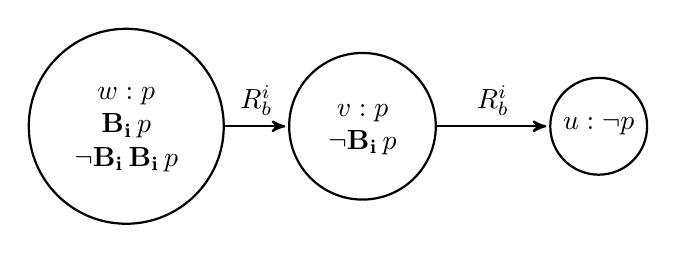
\begin{tikzpicture}[->,>=stealth',shorten >=1pt,auto,node distance=3cm,
		thick,base node/.style={circle,draw,minimum size=35pt}]
		
		\node[base node] (w) {\begin{tabular}{c}
			$w:  p$ \\ $\Bels{i}p$ \\ $\tlnot\Bels{i}\Bels{i}p$
			\end{tabular}};
		\node[base node] (v) [right of=w] {\begin{tabular}{c}
			$v:  p$ \\ $\tlnot\Bels{i}p $
			\end{tabular}};
		\node[base node] (u) [right of=v] {$u: \tlnot p$};
		\path[]
		(w) edge node[above] {$\Rel{b}^i$} (v)
		(v) 
%		edge node[below] {} (w)
		%	\draw [->] (v) edge[in=5,out=355,loop] node[right] {$R$} (v)
		edge node[above] {$\Rel{b}^i$} (u);

		\end{tikzpicture}
	\end{center}
	\caption{A counterexample to $\Bels{i}\varphi\iimplies\Bels{i}\Bels{i}\varphi$.}
\end{figure}

Without positive belief introspection, L\"ob's Theorem for belief is no longer derivable, and therefore this (very weak) epistemic logic avoids L\"ob's Obstacle.

\section{Concluding Remarks}
\label{sec:conclusion}

%
%Frame Condition of Weak Epistemic Restraint
%$(\Rel{k}^i \circ \Rel{b}^i)(w)\bigcap \Rel{b}^i \not= \emptyset$
%for all wv, w rel b v and exists u v rel k u  implies w rel b u
%
%\section{Vingean Reflection}
%How would a reasoner described in Table \ref{GC_agent} perform when reasoning about what ideally rational agents know? To answer this question, we must decide how to represent ideally rational agents. The standard approach is to use an S5 epistemic operator for ideally rational agents. If we do this, and we assume these agents are capable of reasoning about self-referential sentences, then they collapse into inconsistency, which is not characteristic of ideal rationality. Hintikka's weaker S4 epistemic agents also will not do, for the same reason.
%
%A more powerful reasoner should be axiomatizable by a system that can derive the less powerful reasoner
%\paragraph{Paragraph headings} Use paragraph headings as needed.
%\begin{equation}
%a^2+b^2=c^2
%\end{equation}
%
%% For one-column wide figures use
%\begin{figure}
%% Use the relevant command to insert your figure file.
%% For example, with the graphicx package use
%  
\includegraphics{example.eps}
%% figure caption is below the figure
%\caption{Please write your figure caption here}
%\label{fig:1}       % Give a unique label
%\end{figure}
%%
%% For two-column wide figures use
%\begin{figure*}
%% Use the relevant command to insert your figure file.
%% For example, with the graphicx package use
%  
\includegraphics[width=0.75\textwidth]{example.eps}
%% figure caption is below the figure
%\caption{Please write your figure caption here}
%\label{fig:2}       % Give a unique label
%\end{figure*}
%%
%% For tables use
%\begin{table}
%% table caption is above the table
%\caption{Please write your table caption here}
%\label{tab:1}       % Give a unique label
%% For LaTeX tables use
%\begin{tabular}{lll}
%\hline\noalign{\smallskip}
%first & second & third  \\
%\noalign{\smallskip}\hline\noalign{\smallskip}
%number & number & number \\
%number & number & number \\
%\noalign{\smallskip}\hline
%\end{tabular}
%\end{table}


%\begin{acknowledgements}
%If you'd like to thank anyone, place your comments here
%and remove the percent signs.
%\end{acknowledgements}

% BibTeX users please use one of
%\bibliographystyle{spbasic}      % basic style, author-year citations
%\bibliographystyle{spmpsci}      % mathematics and physical sciences
%\bibliographystyle{spphys}       % APS-like style for physics
%\bibliography{}   % name your BibTeX data base

% Non-BibTeX users please use
\begin{thebibliography}{}
%
% and use \bibitem to create references. Consult the Instructions
% for authors for reference list style.
%
\bibitem{RefJ}
% Format for Journal Reference
Author, Article title, Journal, Volume, page numbers (year)
% Format for books
\bibitem{RefB}
Author, Book title, page numbers. Publisher, place (year)
% etc
\end{thebibliography}

\end{document}
% end of file template.tex

